\documentclass[conference, onecolumn]{IEEEtran}

\usepackage[a4paper]{geometry}
\usepackage[T1]{fontenc}
\usepackage{amsmath,amssymb}
\usepackage{array}
\usepackage{booktabs}
\usepackage{graphicx}
\usepackage{xcolor}
\usepackage{tikz}
\usetikzlibrary{arrows.meta,positioning,shapes.geometric}
\usepackage{hyperref}
\usepackage{seqsplit}
\usepackage{placeins}
\hypersetup{
  hidelinks,
  pdftitle={ESV-Gap: A Fail-Closed Evidence Contract for Knowledge-Graph-Based Research-Gap Triage},
  pdfauthor={Hoa Anh Le, Hoang Duc Nguyen, Khoa Ly Van Phan, Thanh Dinh Nguyen},
  pdfkeywords={Research-gap discovery, Knowledge graphs, Perturbation testing, Evidence triage}
}
\usepackage{cite}

\newcommand{\method}{ESV-Gap}
\newcommand{\statuseligible}{\texttt{automatically\_eligible}}
\newcolumntype{L}[1]{>{\raggedright\arraybackslash}p{#1}}

\title{ESV-Gap: A Fail-Closed Evidence Contract for\\
Knowledge-Graph-Based Research-Gap Triage}

\author{
\IEEEauthorblockN{Hoa Anh Le, Hoang Duc Nguyen, Khoa Ly Van Phan, and Thanh Dinh Nguyen}
\IEEEauthorblockA{Department of Information Technology, FPT University, Ho Chi Minh City Campus, Vietnam\\
\{hoalase181702, hoangndse181655, khoaplvse181656, thanhndse182854\}@fpt.edu.vn}
\vspace{0.5em}
\IEEEauthorblockN{\textit{Faculty Supervisor:} Long Truong}
\IEEEauthorblockA{Department of Software Engineering, FPT University, Ho Chi Minh City Campus, Vietnam\\
longt5@fpt.edu.vn}
}

\begin{document}
\maketitle

\begin{abstract}
We present \method{}, a fail-closed triage stage that separates raw graph anomalies from evidence-clear research-gap candidates.
The method canonicalizes entity identity, requires source-disjoint provenance, tests relation-event deletion, paper dropout, and plausible edge addition, normalizes temporal activity, and routes coverage hits to review.
On an 800-candidate controlled fixture test, the evidence contract achieved precision, validator recall, and F1 of 1.000 versus 0.250, 1.000, and 0.400 for the unfiltered baseline; this checks intended implementation behavior rather than real-world gap quality.
On a 185-paper microservices-security snapshot, 256 signals were reduced to 40 review-required items.
A live run on \emph{security of MongoDB} collected 74 records, retained 53, and extracted 643 relation events. A frozen offline gate reduced 128 signals to 9 review-required items. One author-internal reviewer assessed all nine post-gate items, accepting eight and rejecting one (88.9\%). Separately, the same reviewer accepted 24 of 30 candidates (80.0\%) that had been score-ranked before gate application.
TF--IDF retrieval and per-abstract LLM baselines produced 53 and 159 outputs with Jaccard overlaps of 0.1239 and 0.1113 against the score-ranked graph candidates.
These artifacts document workflow operability and a preliminary internal assessment, not validated effectiveness.
\end{abstract}

\begin{IEEEkeywords}
Research-gap discovery, Knowledge graphs, Perturbation testing, Evidence triage.
\end{IEEEkeywords}

\section{Introduction}

Systematic reviews require transparent search, selection, and evidence accounting~\cite{page2021prisma}. Machine learning can accelerate screening and extraction, but automation should expose uncertainty and preserve human oversight~\cite{marshall2019automation,shneiderman2020hcai}. Research-gap discovery is especially sensitive: an omitted relation may reflect a genuinely under-studied question, an abstract-only corpus, an extraction false negative, an unresolved synonym, or a fragmented graph.

A recent preprint generated gap candidates from TransE link prediction, Louvain communities, and temporal decay~\cite{rahul2026dynamic}. Its eight-paper pilot reported 34 graph signals and a 90\% author accept-or-modify rate, while also reporting zero TransE outputs, entity artefacts, and no independent baseline review. The useful insight is structural, but the epistemic interpretation must be narrower: \emph{a graph anomaly is a candidate-generating signal; it is not a validated research gap.}

Our first ESV-Gap implementation enforced provenance, specificity, edge-dropout stability, and lexical retrieval. An internal design audit exposed two defects: a mathematically redundant weighted threshold and single-path fragility. The revised method removes the score from the decision rule, requires source-disjoint path diversity, samples papers as evidence clusters, and tests plausible missing edges.

This paper addresses the following research questions:
\begin{itemize}
  \item \textbf{RQ1:} Can a multi-rule evidence contract reject controlled artefacts across all three signal families (missing link, orphan community, temporal decay) without losing planted positives?
  \item \textbf{RQ2:} Which individual validation components contribute most to artefact rejection, and how sensitive is performance to perturbation parameters?
  \item \textbf{RQ3:} How much does the frozen gate reduce the candidate queue on a real corpus, and does it automatically accept any item?
  \item \textbf{RQ4:} On a live corpus, how do graph-based candidates compare descriptively with TF--IDF retrieval and per-abstract LLM baselines?
  \item \textbf{RQ5:} What does preliminary author-internal review reveal about acceptance rates and signal-family differences?
\end{itemize}

This paper makes four bounded contributions: (1)~an auditable evidence contract distinguishing \statuseligible{}, \texttt{review\_required}, and \texttt{rejected}; (2)~path-specific provenance and multi-mode perturbation testing; (3)~publication-normalized temporal detection with right-censoring and lexical candidate-coverage screening; and (4)~a disjoint-development fixture benchmark, a retrospective real-corpus diagnostic, and a live MongoDB-security run with internal review and descriptive baseline comparisons.

The controlled results demonstrate expected implementation behavior under the authored fixture conditions. They do not establish detector recall, scientific novelty, or real-world precision.

\section{Background and Related Work}

Literature-based discovery predates modern language models: Swanson showed that separately published findings could form testable hypotheses~\cite{swanson1986fish}. Contemporary systematic-review automation addresses search, screening, extraction, and synthesis~\cite{marshall2019automation}. ESV-Gap is closer to evidence triage than autonomous discovery.

Scientific claim verification provides a relevant evaluation model. SciFact couples claims with evidence abstracts~\cite{wadden2020scifact}; SciFact-Open shows that systems evaluated on a small closed corpus degrade in open-domain retrieval~\cite{wadden2022scifactopen}. This motivates our asymmetric rule: a retrieval hit triggers review, while no hit is not proof of absence~\cite{altman1995absence}.

Knowledge graphs support extraction, completion, and reasoning~\cite{schneider2022decade}. TransE treats relations as translations in embedding space~\cite{bordes2013transe}; uncertain KG embeddings retain graded confidence~\cite{chen2019ukge}. Generative extraction can introduce factual inconsistencies~\cite{kim2026graphrefine}. Provenance therefore belongs to relation events, not only nodes, following the spirit of PROV-O~\cite{lebo2013provo}.

Louvain optimizes modularity and can expose communities~\cite{blondel2008fast}, but community structure may be unstable under sampling noise~\cite{karrer2008robustness,abbe2018community}. Stability selection evaluates whether results persist under resampling~\cite{meinshausen2010stability}. Our candidate-level perturbation tests are narrower: they reveal dependence on particular edges, papers, or plausible missing bridges.

\section{Problem Formulation}

Let a temporal literature graph be a directed multigraph
\begin{equation}
G=(V,E), \qquad e=(u,r,v,y,p,q,s),
\end{equation}
where $u,v\in V$ are typed entities, $r$ is a relation, $y$ a publication year, $p$ a paper identifier, $q$ an extraction confidence, and $s$ an evidence span. A detector $D_k$ maps $G$ to candidates $C_k$ of type missing link, orphan community, or temporal decline.

The validator computes an auditable decision
\begin{equation}
\delta(c)\in\{\texttt{automatically\_eligible},\texttt{review\_required},\texttt{rejected}\}.
\end{equation}
The first label means only that the automated evidence contract passed. Novelty, value, and absence from source-complete literature remain human judgments. Conversely, \texttt{rejected} means that the candidate fails the automated evidence contract; it does not mean that the underlying research idea is scientifically invalid or unworthy of human investigation.

\section{Method}

\subsection{Revised Workflow}

\begin{figure}[t]
\centering
\resizebox{\columnwidth}{!}{%
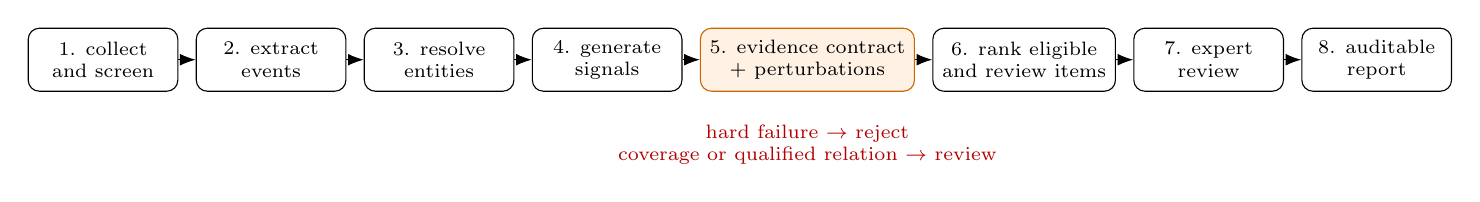
\begin{tikzpicture}[
  node distance=2.2mm,
  box/.style={draw,rounded corners,align=center,minimum height=8mm,minimum width=19mm,font=\scriptsize},
  gate/.style={box,draw=orange!80!black,fill=orange!10},
  arrow/.style={-{Latex[length=2mm]},thin}
]
\node[box] (collect) {1. collect\\and screen};
\node[box,right=of collect] (extract) {2. extract\\events};
\node[box,right=of extract] (resolve) {3. resolve\\entities};
\node[box,right=of resolve] (detect) {4. generate\\signals};
\node[gate,right=of detect] (validate) {5. evidence contract\\+ perturbations};
\node[box,right=of validate] (rank) {6. rank eligible\\and review items};
\node[box,right=of rank] (retrieve) {7. expert\\review};
\node[box,right=of retrieve] (report) {8. auditable\\report};
\foreach \a/\b in {collect/extract,extract/resolve,resolve/detect,detect/validate,validate/rank,rank/retrieve,retrieve/report}
  \draw[arrow] (\a) -- (\b);
\node[below=3mm of validate,font=\scriptsize,text=red!70!black,align=center] {hard failure $\rightarrow$ reject\\coverage or qualified relation $\rightarrow$ review};
\end{tikzpicture}}
\caption{Revised pipeline. Stage 5 separates candidate generation from claims about research gaps.}
\label{fig:pipeline}
\end{figure}

Fig.~\ref{fig:pipeline} inserts the evidence contract before ranking. The implementation keeps parallel relation events so paper-level sampling and temporal normalization remain possible. Every decision serializes metrics, thresholds, seeds, source-paper IDs, evidence paths, coverage hits, and all failed rules.

\subsection{Entity Identity Before Graph Topology}

First, graph construction normalizes Unicode and removes terminal suffixes like \texttt{[METHOD]} or \texttt{[CONCEPT]}. Whitespace is collapsed, and labels differing only by case share an identity key $\kappa(e) = \operatorname{casefold}(\allowbreak\operatorname{stripType}(\allowbreak\operatorname{NFKC}(e)))$. A missing-link pair with $\kappa(h)=\kappa(t)$ is discarded. For coverage retrieval, terminal numeric versions emit a versionless token, e.g.\ \texttt{OAuth2}$\mapsto\{\texttt{oauth2},\texttt{oauth}\}$.

\subsection{Specificity and Path-Specific Provenance}

Let $T(e)$ be the non-stopword tokens in entity $e$ and $g(e)$ the count belonging to a generic vocabulary. The specificity score is
\begin{equation}
q_s(e)=0.75\!\left(1-\frac{g(e)}{\max(|T(e)|,1)}\right)+0.25\min\!\left(\frac{|T(e)|}{3},1\right),
\end{equation}
with threshold 0.55. For a missing-link candidate $(h,t)$, the validator enumerates simple paths of at most four edges and greedily selects paths sharing neither an edge nor a source paper:
\begin{equation}
|\Pi(c)|\geq 2,\qquad P(\pi_i)\cap P(\pi_j)=\varnothing\quad(i\neq j).
\end{equation}
For orphan communities, provenance counts only papers on internal edges; for temporal candidates, papers mentioning the concept. A minimum of two paper IDs is mandatory.

\subsection{Isolation and Normalized Temporal Activity}

For community members $M$, isolation is $I(M)=1-{|E_{\mathrm{cut}}(M)|}/{\max(|E_{\mathrm{in}}(M)|+|E_{\mathrm{cut}}(M)|,1)}$, with threshold $I(M)\geq0.90$.

Raw relation-event counts confound topic activity with corpus growth. We normalize as $a_{v,y}={n_{v,y}}/{\max(N_y,1)}$ over adjacent windows of $L=2$ complete years. When $\bar{a}_H>0$, decay is $d_v=1-{\bar{a}_R}/{\bar{a}_H}$. When $\bar{a}_H=0$, the detector and validation recomputation both assign $d_v=0$: neither zero-to-zero activity nor new activity establishes a decline. A detector signal requires $d_v\geq0.30$. The snapshot date is July 20, 2026; 2026 is right-censored and excluded.

\subsection{Candidate-Coverage Retrieval}

The local screen tokenizes titles and abstracts after type-suffix normalization. Each entity requires at least $\max(1,\lceil0.60|T(e)|\rceil)$ token matches from the canonical label or a declared synonym. A hit routes to review and never hard-rejects a candidate.

\subsection{Multi-Mode Perturbation Stability}

For $B$ deterministic replicates, the signal is tested under three modes: (1)~relation-event retention with probability $\rho$ (deletion probability $1-\rho$); (2)~paper retention with probability $\rho$, where dropping a paper removes all relation events attributed to it; and (3)~plausible edge addition. Thus the frozen value $\rho=0.95$ means 5\% expected deletion/dropout, not 95\%. Over the modes that were actually evaluated, $Q_b(c)=\min_{m\in\mathcal{M}_{\mathrm{eval}}(c)}\frac{1}{B}\sum_{b=1}^{B}I_{b,m}(c)$, with $B=50$ and $Q_b\geq0.70$; availability is enforced separately by the decision rule.

Plausible additions come only from candidate-relevant entries in \texttt{plausible\_edges}, supplied by upstream retrieval or link prediction. Each supplied edge is sampled independently with probability 0.50 per replicate; dictionary-form edges preserve endpoints, relation label, source-paper ID, year, and confidence. Missing-link directness and orphan isolation use endpoint topology without relation-direction matching. Crucially, an empty or irrelevant pool is not treated as survival unless the producer sets \texttt{plausible\_edge\_search\_performed=true}. With that marker, an empty pool means ``searched, no relevant closing edge found'' and the mode survival is 1.0. Without it, the mode is serialized as unavailable (JSON \texttt{null}), and the candidate cannot be automatically eligible.

\subsection{Decision and Ranking}

Insufficient provenance, specificity, path diversity, or stability, and any canonical self-link, is a hard rejection. A coverage hit, observed direct relation, unavailable closure corpus, or unavailable plausible-edge stress test produces \texttt{review\_required} when no hard rule fails. If no hard or review condition fires, the label is \statuseligible{}. The gate decision $\delta(c)$ is computed before ranking; ranking orders only post-gate survivors for expert review. Evidence metrics are combined as $R(c)={\sum_{j\in A(c)}w_jq_j(c)}/{\sum_{j\in A(c)}w_j}$ with $w=(.25,.15,.20,.30,.10)$. Changing $R(c)$ cannot change $\delta(c)$.

\section{Experimental Design}

This section describes the three experimental settings used to address RQ1--RQ5.

\subsection{Disjoint Controlled Benchmark}

The generator creates 16 candidates per seed: four positives and twelve negatives spanning missing-link, orphan, and temporal signal types. Every fixture explicitly marks its candidate-level plausible-edge search as completed; empty fixture pools therefore represent completed searches with no relevant edge, rather than missing tests. Ten seeds are reserved for a 48-cell sensitivity grid (see Appendix~\ref{app:sensitivity}). Parameters are frozen before evaluation on 50 disjoint test seeds: 800 candidates, 200 positive. We compare retaining every signal, single-component gates, the hard contract without perturbation, and the full contract.

The binary evaluation mapping is explicit. Ground truth is $y=1$ only for a planted evidence-sufficient candidate and $y=0$ for a planted artefact or covered/qualified candidate. The gate prediction is $\hat y=1$ only for \statuseligible{}; both \texttt{review\_required} and \texttt{rejected} map to $\hat y=0$. Thus TP, FP, TN, and FN count $(y,\hat y)=(1,1),(0,1),(0,0),(1,0)$, respectively. This mapping evaluates automatic eligibility, not whether a reviewer might later accept a review-required item.

\subsection{Retrospective Corpus Diagnostic}

The inherited snapshot contains 185 microservices-security papers and 1,018 provenance-rich relation events spanning 2018--2026. We run deterministic common-neighbour missing-link generation (top~50), fixed-seed Louvain, and normalized temporal decay. This is a retrospective diagnostic, not a reproducible PRISMA construction. Details are in Appendix~\ref{app:corpus}.

\subsection{Live MongoDB-Security Execution}

On August 6, 2026, we ran the deployed Streamlit application with the topic \emph{security of MongoDB} and a maximum budget of 100 papers. This run is labeled ``corrected'' because it followed an earlier diagnostic in which a topic-mismatched screening prompt retained only four of 150 papers. The present run uses a topic-conditioned prompt and is followed by a separate offline evaluation using the frozen evidence-contract gate. The run directory \texttt{security\_of\_mongodb\_20260806\_135447} preserves all artifacts. The Groq-hosted \texttt{llama-3.1-8b-instant} model was used for screening, extraction, and generation. Missing-link generation used the deterministic common-neighbour fallback because PyKEEN was unavailable.

B1 (TF--IDF retrieval + LLM baseline) retrieves the three most similar abstracts via TF--IDF cosine and generates one structured remaining-gap output per paper. B2 (no-retrieval per-abstract LLM baseline) requests three gaps per paper. Both use the same 53-paper corpus and model. The reported Jaccard value is descriptive: for each method, outputs are lowercased and split on whitespace, tokens are pooled across the corpus, and overlap is computed between the resulting token sets. ``Unique'' denotes exact output-string uniqueness, and mean length uses the same whitespace tokenization. These measures do not evaluate correctness, novelty, or usefulness.

One reviewer (\texttt{author\_internal}) used Accept/Reject/Modify/Pending for two explicitly separated queues. The first comprised the top 30 score-ranked graph candidates selected before gate application. The second comprised all nine post-gate \texttt{review\_required} candidates; one candidate appears in both queues. Both artifacts contain categorical decisions but no item-level rationales, and their overall-notes fields are empty. The reviews were not blinded, had no second reviewer or adjudication, and did not include B1/B2 outputs. They document reviewer disposition and interface persistence, not novelty, precision, or independent external-expert validation.

\section{Results}

\subsection{Controlled Classification and Ablation}

\begin{table}[t]
\caption{Held-out controlled test (800 candidates; 200 positives).}
\label{tab:controlled}
\centering
\begin{tabular}{lrrrrrrr}
\toprule
Method & TP & FP & TN & FN & Prec. & Rec. & F1\\
\midrule
Retain every signal & 200 & 600 & 0 & 0 & .250 & 1.000 & .400\\
Full evidence contract & 200 & 0 & 600 & 0 & 1.000 & 1.000 & 1.000\\
\bottomrule
\end{tabular}
\end{table}

\begin{table}[t]
\caption{Ablation on the held-out test.}
\label{tab:ablation}
\centering
\begin{tabular}{lrrrr}
\toprule
Configuration & FP & Precision & Recall & F1\\
\midrule
Provenance only & 550 & .267 & 1.000 & .421\\
Specificity only & 550 & .267 & 1.000 & .421\\
Path diversity only & 500 & .286 & 1.000 & .444\\
Perturbation only & 350 & .364 & 1.000 & .533\\
Hard contract, no perturb. & 300 & .400 & 1.000 & .571\\
Full, no coverage & 100 & .667 & 1.000 & .800\\
Full evidence contract & 0 & 1.000 & 1.000 & 1.000\\
\bottomrule
\end{tabular}
\end{table}

Table~\ref{tab:controlled} shows that, within the authored fixture generator, the full contract removed all 600 planted negatives without losing a planted positive. Table~\ref{tab:ablation} shows that no single rule explains this fixture result: coverage retrieval removes the remaining synonym-coverage negative class, while source-disjoint paths and perturbations address different planted dependence failures. Sensitivity analysis and ranking metrics are in Appendix~\ref{app:sensitivity}.

\subsection{Real-Corpus Triage}

\begin{table}[t]
\caption{Frozen-gate outcome on the 185-paper snapshot.}
\label{tab:real}
\centering
\begin{tabular}{lrrrr}
\toprule
Signal & Raw & Eligible & Review & Reject\\
\midrule
Missing link & 50 & 0 & 14 & 36\\
Orphan community & 194 & 0 & 17 & 177\\
Temporal decay & 12 & 0 & 9 & 3\\
\midrule
Total & 256 & 0 & 40 & 216\\
\bottomrule
\end{tabular}
\end{table}

Table~\ref{tab:real} shows a reduction from 256 detector signals to 40 review-required items, an 84.4\% candidate-queue reduction. No item is \statuseligible{}. The five items previously assigned that label were artifacts of entity identity or coverage tokenization that the revision corrected.

\subsection{Live-Run Outputs and Baselines}

The live run collected 74 unique Semantic Scholar records across five queries, retained 53 (71.6\%), extracted 643 relation events, and built a 578-node, 636-edge graph with 61 weak components. Detectors emitted 128 raw signals (50 missing-link, 71 orphan, 7 temporal).

\begin{table}[t]
\caption{Evidence-contract gate outcome on the 53-paper live corpus.}
\label{tab:live_gate}
\centering
\begin{tabular}{lrrrr}
\toprule
Signal & Raw & Eligible & Review & Reject\\
\midrule
Missing link & 50 & 0 & 0 & 50\\
Orphan community & 71 & 0 & 3 & 68\\
Temporal decay & 7 & 0 & 6 & 1\\
\midrule
Total & 128 & 0 & 9 & 119\\
\bottomrule
\end{tabular}
\end{table}

Table~\ref{tab:live_gate} shows the frozen gate reduced 128 raw signals to 9 review-required candidates, a 93.0\% candidate-queue reduction. No item is \statuseligible{}. All 128 preserved detector candidates predate the plausible-edge-search completion marker, so the addition mode is recorded as unavailable for each rather than as survived; the nine candidates that pass the hard rules therefore remain review-required. All 50 missing-link candidates were rejected, primarily due to insufficient source-disjoint paths in a 53-paper corpus. All nine post-gate items were subsequently reviewed; the pre-gate score-ranked top 30 form a separate, partly overlapping review cohort.

\begin{table}[t]
\caption{Descriptive baseline comparison on the 53-paper corpus.}
\label{tab:baselines}
\centering
\begin{tabular}{L{3.0cm}rrrr}
\toprule
Method & Outputs & Unique & Mean words & Jaccard vs KG\\
\midrule
KG candidate ranker & 30 & 30 & 27.6 & 1.0000\\
B1: TF--IDF retr.\ + LLM & 53 & 53 & 67.2 & 0.1239\\
B2: per-abstract LLM & 159 & 159 & 28.9 & 0.1113\\
\bottomrule
\end{tabular}
\end{table}

\begin{table}[t]
\caption{Complete author-internal review of the post-gate queue.}
\label{tab:postgate_review}
\centering
\begin{tabular}{lrrr}
\toprule
Signal & Shown & Accept & Reject\\
\midrule
Orphan community & 3 & 3 & 0\\
Temporal decay & 6 & 5 & 1\\
\midrule
Total & 9 & 8 & 1\\
\bottomrule
\end{tabular}
\end{table}

\begin{table}[t]
\caption{Preliminary author-internal review of ranked graph candidates.}
\label{tab:review}
\centering
\begin{tabular}{lrrrrr}
\toprule
Signal & Shown & Accept & Modify & Reject & Pending\\
\midrule
Missing link & 4 & 0 & 0 & 4 & 0\\
Orphan community & 25 & 23 & 0 & 2 & 0\\
Temporal decay & 1 & 1 & 0 & 0 & 0\\
\midrule
Total & 30 & 24 & 0 & 6 & 0\\
\bottomrule
\end{tabular}
\end{table}

Table~\ref{tab:baselines} shows low Jaccard overlap between graph candidates and both baselines. Together with the length differences, this is consistent with different vocabulary and output granularity, but it does not demonstrate superiority. B1--B2 overlap was 0.3333. No shared external-expert labels are available.

All 30 items in Table~\ref{tab:review} received a decision: 24 were accepted (80.0\%) and six rejected. No item remained Modify or Pending. All four missing-link items were rejected, whereas 23 of 25 orphan-community items and the single temporal item were accepted. These proportions describe only this selected review queue.

All nine post-gate items in Table~\ref{tab:postgate_review} also received a decision: eight were accepted (88.9\%) and one was rejected, with no Modify or Pending label. The reviewer accepted all three orphan-community items and five of six temporal-decay items; the rejected item was the \emph{Cloud infrastructure} temporal signal. Because the gate intentionally routes uncertain items for judgment, ``Accept'' means retain for follow-up, not that a source-complete literature gap was proven.

\begin{table}[t]
\caption{Cross-tabulation of gate outcome versus author-internal review for the 30 score-ranked candidates.}
\label{tab:crosstab}
\centering
\begin{tabular}{lrrrr}
\toprule
Gate outcome & Accept & Modify & Reject & Pending\\
\midrule
Review required & 1 & 0 & 0 & 0\\
Rejected & 23 & 0 & 6 & 0\\
Automatically eligible & 0 & 0 & 0 & 0\\
\bottomrule
\end{tabular}
\end{table}

Table~\ref{tab:crosstab} contrasts the gate's decision with the internal reviewer's assessment. The gate and reviewer now agree in rejecting all four displayed missing-link candidates, but the reviewer accepted 23 other candidates that the gate rejected. The two labels use different criteria: gate rejection records failure of at least one automated evidence-contract rule, whereas the review artifact records a categorical disposition without a preserved rationale. Their disagreement identifies items for independent assessment but does not establish false negatives. Because the 30 reviewed candidates were selected by pre-gate score ranking rather than random or stratified sampling, this cross-tabulation is selection-biased and cannot estimate the gate's population false-negative rate.

\section{Discussion}

Entity identity precedes topology: treating type suffixes as lexical content created artificial nodes and broke coverage screening. Source-disjoint paths expose single-source dependence. Paper dropout respects correlation among events from the same document. Plausible edge addition tests extraction false negatives.

The gate's behavior on the live corpus is directionally similar to the retrospective snapshot: 93.0\% rejection on 128 signals versus 84.4\% on 256, with zero automatically eligible items in both. The smaller corpus may contribute to the higher rejection rate because fewer papers can supply source-disjoint paths, but the two corpora differ in topic and construction, so the cause is not identified. In this run, every common-neighbour missing-link candidate failed the source-disjoint-path requirement; this observation should not be generalized to other graphs or link predictors.

The complete post-gate review is aligned with the operational queue: one unblinded internal reviewer accepted eight of nine items (88.9\%). It is still not an estimate of precision because the reviewer was not independent, no rationale or source-complete search was preserved, and the queue was constructed specifically from uncertain survivors. The separate 80.0\% pre-gate acceptance rate likewise describes disposition only. The 23 Accept decisions among 29 gate-rejected displayed items may indicate that the hard gate is conservative, but the selected sample cannot quantify under-retention. A useful follow-up would obtain shared, blinded expert labels for gate survivors, a stratified sample of rejections, B1, and B2 candidates. The low Jaccard overlap motivates but does not substitute for that comparison.

Perfect controlled performance should invite caution: the generator is authored with knowledge of the evidence contract and tests implementation behavior, not generalization to naturally occurring gaps.

\section{Limitations}

The real corpus is abstract-only, single-domain, and retrospectively inherited. The live run used a single Groq-hosted 8B model for all LLM stages, TF--IDF fallback for B1, and common-neighbour fallback for link prediction. The same internal author reviewed the top 30 pre-gate candidates and all nine post-gate candidates; the cohorts overlap by one item and are not independent samples. The reviewer was unblinded, supplied no item-level rationales, and had no second reviewer or adjudication; B1/B2 were not in either review packet. Coverage retrieval is lexical and does not verify relation direction, polarity, or outcome. The greedy path selector is deterministic but is not guaranteed to find a maximum source-disjoint path set, so it may conservatively reject candidates for which a better path packing exists. Entity merge/split perturbation, full-text retrieval, and citation chasing remain future work. Distinct papers are not necessarily independent studies. The controlled benchmark's perfect result must not be read as evidence that the system discovers true gaps perfectly.

\section{Conclusion and Future Work}

\method{} treats graph anomalies as hypotheses and makes the evidence contract explicit. On an 800-candidate controlled test it rejected every planted artefact (RQ1); this is an implementation-validity result. Ablation showed that no single rule suffices within those fixtures; coverage retrieval, source-disjoint paths, and perturbation address distinct planted failure modes (RQ2). On a 185-paper retrospective snapshot the gate reduced 256 signals to 40 review-required candidates with none automatically eligible, an 84.4\% candidate-queue reduction (RQ3). On the 53-paper MongoDB live corpus the same frozen gate reduced 128 signals to 9 review-required items (93.0\% reduction), again with none automatically eligible; TF--IDF retrieval and per-abstract LLM baselines produced 53 and 159 outputs with Jaccard overlaps of 0.1239 and 0.1113 against the score-ranked graph candidates (RQ4). One author-internal reviewer accepted eight of all nine post-gate items (88.9\%); separately, the same reviewer accepted 24 of 30 pre-gate score-ranked items (80.0\%) (RQ5). Because no shared external-expert labels exist and neither review was blinded or independent, the live artifacts document workflow operability and reviewer disposition, not validated or comparative effectiveness.

Future work includes: (1)~a preregistered, multi-domain, blinded expert study evaluating both gate-surviving and gate-rejected candidates; (2)~replacing the common-neighbour fallback with trained link-prediction models (e.g., TransE, RotatE); (3)~extending coverage retrieval to full-text and citation-chasing; (4)~entity merge/split perturbation and extraction-model reruns; and (5)~multi-reviewer adjudication with inter-rater reliability metrics.

\section*{Acknowledgements}
The authors thank FPT University for supporting this research. The authors have no competing interests to declare.

The \href{https://github.com/Khoa-Hoa-Technology-Solution-Company/research-paper-gap}{project repository is hosted on GitHub}. A checksum-addressed archive distributed with the submission freezes the executable validator, configuration, inputs, outputs, tests, and manifest. Its filename and digest, sensitivity analysis, corpus integrity audit, and expert evaluation protocol are in the appendices.

\FloatBarrier
\bibliographystyle{IEEEtran}
\bibliography{references}

%% ===== APPENDICES (not counted in 10-page limit) =====
\appendices

\section{Sensitivity Analysis and Ranking}
\label{app:sensitivity}

Across the 48 development configurations ($\rho\in\{0.70,0.80,0.90,0.95\}$, $B\in\{50,100,200\}$, $\tau\in\{0.70,0.80,0.90,0.95\}$), fixture F1 ranged from 0.462 to 1.000; seven cells reached 1.000. Mean F1 rose from 0.549 at $\rho=0.70$ to 0.940 at $\rho=0.95$. Increasing $B$ from 50 to 200 changed mean F1 from 0.722 to 0.752, while increasing the threshold from 0.70 to 0.95 reduced mean F1 from 0.873 to 0.625. We selected the lowest-cost configuration reaching fixture F1=1.000, $(\rho,B,\tau)=(0.95,50,0.70)$, before opening test results.

For diagnostic purposes, the following ranking experiment is computed over all 800 pre-gate candidates to evaluate score separation; operational ranking in the benchmark applies only to post-gate survivors. At matched budget $k=200$, detector-score ranking achieved average precision 0.153. Evidence-score ranking achieved Precision@200 and Recall@200 of 0.770, nDCG@200 of 0.816, and average precision of 0.906. Equal, provenance-heavy, and path-heavy schemes shared nDCG@200 of 0.816; specificity-heavy obtained 0.704.

\section{Corpus Integrity Audit}
\label{app:corpus}

The inherited microservices-security snapshot contains 185 papers with 1,018 provenance-rich relation events. A reproducible audit found 185 unique paper IDs, abstracts for every record, 184 DOI-bearing records (all returning resolver redirects on August 5, 2026), and 989 of 1,018 evidence quotes (97.15\%) as exact case-insensitive substrings of recorded abstracts. The remaining 29 quotes are flagged as extraction risks. The current gate does not independently verify quote-text alignment, so this audit flag must not be interpreted as a gate decision.

Events record the model identifier
\texttt{ram/\allowbreak gemini-\allowbreak 3.5-flash-low}
and prompt version
\texttt{triple-\allowbreak extraction-\allowbreak v2-\allowbreak provenance},
along with a prompt SHA-256, request timestamps, evidence spans, and paper IDs.
Canonicalization reduced the graph from 1,149 raw labels to 1,130 entity nodes; the resulting multigraph contains 1,018 events and 176 weak components.

\section{Artifact Contract}
\label{app:artifact}

\begin{table}[h]
\caption{Artifact contract at the time of this revision.}
\label{tab:artifact}
\centering
\begin{tabular}{L{3.2cm}L{8.0cm}}
\toprule
Field & Value\\
\midrule
Repository & \href{https://github.com/Khoa-Hoa-Technology-Solution-Company/research-paper-gap}{GitHub: Khoa-Hoa-Technology-Solution-Company/research-paper-gap}\\
Live run & \texttt{security\_of\_mongodb\_20260806\_135447}; 74 collected, 53 retained, 643 relation events, 128 raw detector signals, and 30 ranked.\\
Submission archive & \path{esv-gap-final-20260810-r1.zip}; 43 manifest-tracked files; offline reproduction requires no API key.\\
Runtime & CPython 3.14.6\\
\bottomrule
\end{tabular}
\end{table}

The controlled benchmark report SHA-256 is \seqsplit{9796cbcdd08b7a13e60b8a37eea8cbd5a8418feb2c845a5e852fe5e6ecb2e4fe}. Live-run SHA-256 values:
\begin{itemize}
  \item filtered corpus: \seqsplit{1f47c496466ce241b72330c9a80ceaf384de683f8af49b98bc30b75e7d244853};
  \item extracted triples: \seqsplit{bf17038593413d26c60b1a8d781ed1d5ad580722c8d93542be2cba4b176a0386};
  \item raw detector output: \seqsplit{3af4d23f82ab1e3c7200825743ecce9b2f418bfcdc4ff6c6591997ce4cc51d12};
  \item live gate report: \seqsplit{06eadc23301857b636378cdd8a0e236b08df94937a688a9f91e44b3564e2f46d};
  \item ranked top-30: \seqsplit{9cd92844fb48d24534b484838c3b1c4946eb6bb737b7edeb48d3657c58d506e2};
  \item pre-gate author-internal review: \seqsplit{02a355a757f67f7af1aef9b08c13363d7a73c8d5f285f7d1f1252f5671cbec64};
  \item post-gate author-internal review: \seqsplit{390b91827507a27383a3c972b90e81425cbd44f921b2ac5cdc87e791b84e18aa};
  \item baseline comparison: \seqsplit{ecee805edf656c6bb043be39846e50a7eb5e729ed359a03908c2a712cadfe25e};
  \item B1 output: \seqsplit{582e860e1dd7ce17bd1884c060fa2215027e5bd4602173d49fdf48d4a00990ba}; and
  \item B2 output: \seqsplit{e3047e3d160e138353f8ff65deed7c66d52118b18a0d02abd45e299049f3a862}.
\end{itemize}

The frozen gate was reproduced from the archived graph, detector output, and 53-paper screened corpus with the exact command:
\begin{center}
\small\texttt{python reproduce\_frozen\_validation.py}\\[-1pt]
\texttt{-{}-config frozen\_validation\_config.yaml}
\end{center}
The resulting summary was 128 raw, zero automatically eligible, nine review-required, and 119 rejected; its report hash is listed above. The archive SHA-256 is \seqsplit{c6e3d3daf7959598b68b386d39fb8af4126a1d98e7d314e64b239cd07483c835}; \path{MANIFEST.sha256} verifies every file inside the archive.

\section{Expert Evaluation Protocol}
\label{app:expert}

No independent external-expert ratings are reported. One unblinded internal author completed both live-run queues: 8/9 Accept on the post-gate queue and 24/30 Accept on the pre-gate ranked queue, with one overlapping item and no written rationales. For a future evaluation on the inherited microservices corpus, the preparation artifact creates a 70-item blinded packet (40 non-rejected + 30 stratified rejected). At least three domain experts should independently rate source support, novelty, importance, actionability, and feasibility. Reviewers should be blinded to system status. With an explicitly defined consensus rule, the analysis could then estimate expert-judged precision on non-rejected items, a sampled rejection error rate, usefulness, time per candidate, and Krippendorff's alpha. These quantities are protocol targets, not results of the present study.

\section{Audit Case Studies}
\label{app:cases}

\begin{table}[h]
\caption{Representative audit outcomes.}
\label{tab:cases}
\centering
\begin{tabular}{L{2.3cm}L{4.0cm}L{5.0cm}}
\toprule
Outcome & Candidate & Auditable reason\\
\midrule
Rejected & AWS API Gateway--Security & Only one source-disjoint path; 28 local co-mentions cannot repair insufficient provenance.\\
Review required & Docker--Kubernetes & Hard checks pass, but five abstracts co-mention the concepts.\\
Removed self-link & Scalability variants & Type suffixes and case are metadata; both labels canonicalize to the same entity.\\
Review required & JWT--OAuth & Two source-disjoint paths pass, but nine abstracts co-mention normalized labels.\\
\bottomrule
\end{tabular}
\end{table}

\end{document}
